%!TEX root = ../notes.tex
\section{March 25, 2022}
\subsection{Quantum Computation}
\emph{Warm-up:} Deutch's Algorithm

\ul{Setup}: We have a function $f : \{0, 1\}\to \{0, 1\}$. We note there are 4 possibilities for functions $f$. Let's say we have a black box that takes $x$ and computes $f(x)$, taking an hour to run.

Our question is ``is $f$ constant''? Does $f(0) = f(1)$?

Classically, the fastest algorithm takes $2$ hours. We pass in $0$ and then pass in $1$ and check if they are equal.

At the end, we know $f(0) \overset{?}{=} f(1)$. But we know more! We know exactly what $f(0)$ and $f(1)$ are.

\ul{Quantum Reformulation}: we can \emph{manipulte quantum states}. We consider the simplest system, an electron $e^-$. An electron has a property called \emph{spin}: which can be in one of two states:
\[\Ket{\uparrow}, \quad \Ket{\downarrow}\]
which we notate $0$ and $1$.

\begin{remark*}
    The state of the system is \textbf{not a ``probabilistic classical state''.}. It's \textbf{not} represented as
    \[a\cdot \Ket{\uparrow} + b\cdot \Ket{\downarrow}\]
    where $a, b$ are positive reals with $a + b = 1$.
\end{remark*}

The \emph{actual state} of our machine is
\[a\cdot \Ket{\uparrow} + b\cdot \Ket{\downarrow}\]
where $a, b\in\CC$ where $|a|^2 + |b|^2 = 1$. The probability of measuring $\Ket{\uparrow}$ is $|a|^2$ and $\Ket{\downarrow}$ is $|b|^2$.

\begin{example}
    The typical experiment for this is the light passing through two slits:
    \begin{center}
        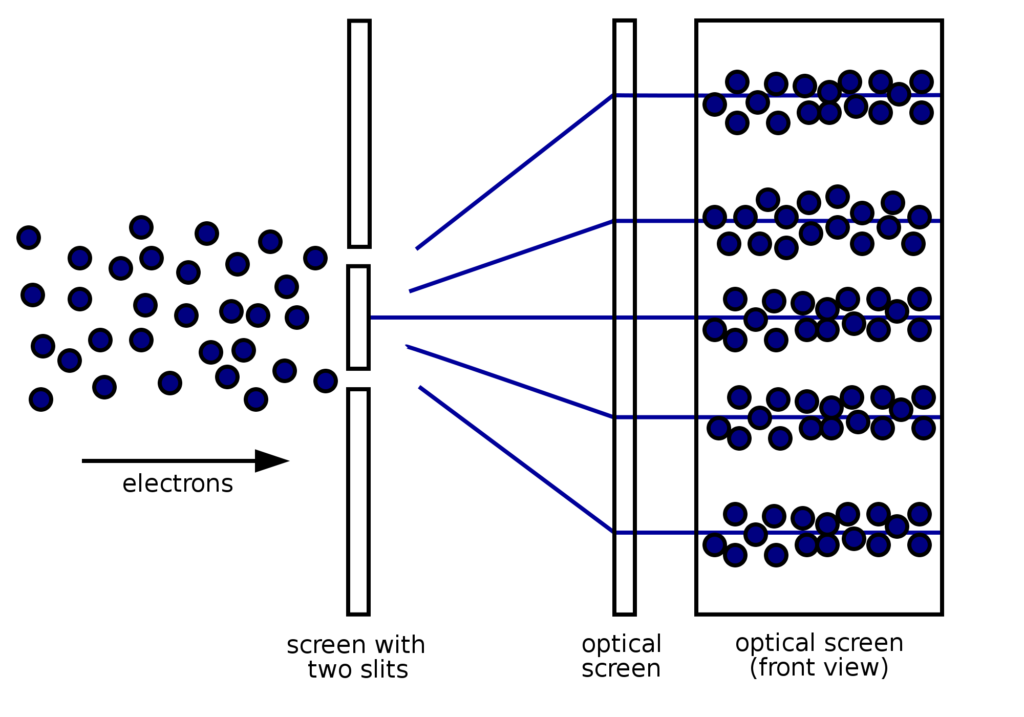
\includegraphics[width=0.5\textwidth]{images/slit-experiment.png}
    \end{center}
\end{example}

We'll run black box again with quantum mechanics - except we only run it once and don't require the knowledge of what $f(0)$ and $f(1)$ \emph{actually are}.

The laws of quantum mechanics are time symmetric. Thus,
\[f : \begin{cases}
        0\mapsto 0 \\
        1\mapsto 0
    \end{cases}\]
\emph{cannot} exist in a quantum computer since it's not invertible. How do we encapsulate our function to be run in a quantum computer?

We define a new function
\[F(x, y) = (x, f(x) + y \text{ mod } 2)\]
$F$ and $f$ encode exactly the same information. But $F$ is defined in a way such that it fits on a quantum computer since it's an invertible function. Classically, it makes no difference having a box that computes $F$ or a box that computes $f$. Computing one gives us the other.

\subsubsection{Deutch's Problem}
Given a \emph{quantum} black box for $F$. Can we determine whether $f(0) = f(1)$?

The idea is that we feed in $x$ and $y$ as superpositions between $0$ and $1$ and exploit cancellation. We evaluate
\begin{align*}
     & \phantom{=} F\left( \frac{1}{\sqrt{2}}\Ket{0}+\frac{1}{\sqrt{2}}\Ket{1}, \frac{1}{\sqrt{2}}\Ket{0} - \frac{1}{\sqrt{2}}\Ket{1} \right)                                \\
     & = \frac{1}{2} \Ket{0}\otimes \Ket{f(0)} - \frac{1}{2}\Ket{0}\otimes \Ket{f(0) + 1} + \frac{1}{2}\Ket{1}\otimes \Ket{f(1)} - \frac{1}{2}\Ket{1} \otimes \Ket{f(1) + 1} \\
     & = \frac{1}{2}\boxed{\left( (-1)^{f(0)}\Ket{0} + (-1)^{f(1)}\Ket{1} \right)}\otimes \left( \Ket{0} - \Ket{1} \right)
\end{align*}

What if I measure the first register? We get $50\%$ chance of $\Ket{0}$ and $50\%$ chance of $\Ket{1}$ and we gain no information.

Graphing this, we have $4$ states $(1,1)$, $(-1, -1)$, $(1, -1)$, and $(-1, 1)$. Applying a rotation matrix
\[\begin{pmatrix}
        \frac{1}{\sqrt{2}}  & \frac{1}{\sqrt{2}} \\
        -\frac{1}{\sqrt{2}} & \frac{1}{\sqrt{2}}
    \end{pmatrix}\]
we get states on the axes. So we get $\Ket{1}$ if $f(0) = f(1)$ and $\Ket{0}$ if $f(0) \neq f(1)$.